\chapter{实验与评测}\label{ch:experiments}

本章检查系统能否形成正式数据产品、能否保留来源与处理记录，以及与通用智能体环境相比交付了哪些内容、花费多少时间和模型用量。实验包括十案例汇总与两个案例的跨环境观察。每个列示条件只有一次运行，不据此估计稳定成功率，也不作单项机制的因果判断。

\section{评测问题与方法}\label{sec:eval-protocol}

十个案例覆盖表达组学、变异、靶点证据、蛋白结构、生物活性、论文图表、GWAS、药物安全、罕见病和微生物组。系统接收研究任务，记录起止时间、模型用量、工具调用、人工确认与终态。一次任务提交到终态计为一个运行单元，内部重试不另计。本文汇总不同批次的十二次运行，不将其写成同一代码和提示配置下的统一试验。

其中，样例6—10的 flash 运行与样例6的 max 运行来自已归档的六运行批次，使用代码提交 \code{e5aadfe0}\cite{biomed-evidence}。样例6使用冻结的任务与执行上下文；样例7、8、10使用重建的历史任务提示；样例9从历史事件恢复原始输入。样例6 max 的完整标识为 \code{qwen3.8-max-0902}，并使用修正模型元数据后的代理运行环境。以上差异保留在运行记录中，不归因于模型档位本身。

评测分开记录三类结果。正式发布状态说明文件是否通过配置的发布检查；需求完成情况说明原始任务中哪些内容已经取得、哪些仍有缺口；运行成本记录时间、token 和工具调用。来源标注、记录定位、清单、方法、质量检查及原始材料则用于判断结果能否进一步复核。文件摘要一致只说明交付文件与记录相符。

十个案例各列示一次 qwen3.8-flash 运行，样例1与样例6另列一次 max 运行。样例1的两个环境做过共有记录抽样互查，但未对照原始来源。本轮没有给出来源级数值正确率、独立参考集召回率或冻结输入后的重跑一致率；这些指标不能由发布率或哈希通过率代替。

\textbf{实验材料。}六运行批次的起止事件、token 分项、工具计数和发布摘要见仓库 \path{docs/evaluation/gold6-10-2026-09-03/}；Qoder 样例6离线包的复核结果见 \path{docs/evaluation/gold6-qoder-2x2/}。这些材料支持各自范围内的核对，不包含全部跨环境计时和用量原始记录。Qoder 时间与 token 沿用人工记录，仅作为描述值保留，不据此计算费用或声称同等工作量下的效率收益。

\section{十案例总体表现}\label{sec:gold-overview}

\subsection{完成情况与数据产品}

表~\ref{tab:gold-overview}汇总每个案例的 flash 运行。样例1—9至少形成一次正式发布，样例10因必需数据未满足条件而停止。表中“成功发布”是运行状态，不表示原始需求全部完成；多次发布与多件文件也不重复计为成功案例。

\begin{xltabular}{\linewidth}{>{\hsize=0.43000\hsize}L>{\hsize=1.25000\hsize}L>{\hsize=0.67000\hsize}L>{\hsize=1.78000\hsize}L>{\hsize=0.87000\hsize}L}
\caption{十案例运行结果与实际交付内容}\label{tab:gold-overview}\\
\toprule
\textbf{案例} & \textbf{研究任务} & \textbf{发布状态} & \textbf{已交付内容与范围} & \textbf{时长 / token} \\
\midrule
\endfirsthead
\toprule
\textbf{案例} & \textbf{研究任务} & \textbf{发布状态} & \textbf{已交付内容与范围} & \textbf{时长 / token} \\
\midrule
\endhead
样例1 & 乳腺癌肿瘤与正常组织转录组整合 & 成功发布 & GSE86374 表达长表，GPL6244 探针映射，5,294,223行 & 26 min / 5,952 K \\
样例2 & LUAD EGFR 突变表达双层级整合 & 成功发布 & GSE31547 探针级与基因级双发布，各1,114,150行 & 23 min / 10,999 K \\
样例3 & EGFR NSCLC 靶点多源证据整合 & 成功发布 & 靶点证据11行、结构6行、药物活性100行，分别发布 & 12 min / 3,818 K \\
样例4 & Spike–ACE2 结构、序列与变异证据 & 成功发布 & 五表：结构2行、病毒蛋白2行、Spike变异110行、界面残基119行、文献2行 & 61 min / 9,916 K \\
样例5 & EGFR 抑制剂活性与化合物结构整合 & 成功发布 & ChEMBL活性与化合物交叉对照双发布，各100行 & 14 min / 2,493 K \\
样例6 & EGFR 突变体抑制实验与论文证据 & 成功发布 & 六张表及表结构、溯源与质量评估，共九件；需求逐项比较见\ref{subsec:gold6-artifact-compare} 节 & 98.9 min / 6,915 K \\
样例7 & 阿尔茨海默病 GWAS 风险位点整合 & 成功发布 & 风险位点与变异—基因映射分别发布 & 36.2 min / 6,350 K \\
样例8 & 药物性肝损伤风险药物证据整合 & 成功发布 & FAERS断言与研究数据；其他请求维度仍为暂存结果 & 45.9 min / 10,646 K \\
样例9 & 原发性免疫缺陷基因—疾病证据整合 & 成功发布 & 动态基因—疾病证据产品，共五件；不同于原静态四表规格 & 351.2 min / 8,529 K \\
样例10 & 肠道微生物组—疾病关联整合 & 未发布 & 两次执行分别因必需分类映射表、差异丰度表为空而拒绝，无正式产物 & 108.5 min / 23,168 K \\
\bottomrule
\end{xltabular}

来源、发布文件与原始需求需要分别检查。例如样例8只正式交付 FAERS 断言与研究数据，其余要求仍未形成正式产品；样例9转向动态规格后取得发布结果，但不能据此认定原静态四表要求已经全部满足。表~\ref{tab:gold-overview}保留这些运行的发布状态，同时说明交付范围。

从产品形态看，系统既能处理数百万行表达数据，也能组织结构、活性和疾病证据等多表产品。样例3–5展示了跨数据库实体对齐，样例7 和样例9 展示了运行时表结构对开放来源集合的适配。样例10 虽未完成交付，但终态和阻断原因均被明确记录，说明发布判定取决于正式数据产品，而不是模型的自然语言声明。样例4 的文献表仅2 行，反映该次运行对该主题只采集了少量文献证据，其检索范围以运行记录为准。

样例10的两次执行分别因必需分类映射表和差异丰度表为空而拒绝。部分候选文件已暂存，但未满足四表同时完整的要求，因此任务没有完成。该结果说明此次发布检查阻止了不完整文件进入正式交付；它不能区分来源本无数据与系统检索、解析不足。改进需要先核查缺失来源，再决定补充解析器还是允许显式标注范围的部分交付。

\subsection{运行成本与人工确认}\label{sec:corrected-six-run}

十二个列示运行中，十一个形成正式发布物，一个未发布，运行级正式发布比例为91.7\%。其中，已归档六运行批次为5/6，即83.3\%。两者分母不同，不能互换；由于任务与配置不同，这些比例用于汇总观察结果，不作为模型成功概率或原始需求完成率。

运行成本方面，flash 运行的耗时介于12–351.2 分钟、token 消耗介于2.5M–23.2M：样例9 用时最长（351.2分钟）；样例10 的token 消耗最高（23.2M），工具调用达264 次，但因必需数据缺失，最终保持未发布。两次max 运行分别耗时30 分钟（样例1）与78 分钟（样例6）。模型调用方面，样例7–9 的flash 运行为40–66 次模型调用、65–88 次工具调用；样例6 max 仅用29 次模型调用和54 次工具调用完成发布，少于同案例flash运行的41 次与71 次。

汇总记录中，样例6 flash 与 max 分别有5次、4次业务 HIL，其余运行没有此类请求。flash 的5次包括3次来源访问授权和2次发布验收。请求次数不自动等于人工实际操作次数，模型初审与人工处理应分别记录；样例7、样例9没有业务 HIL，因此本轮不能用它们验证动态发布强制人工验收。

这些记录让研究者能够区分正式发布与未发布，观察长任务在哪些步骤消耗时间，并检查是否出现审批。它们不能代替独立的内容正确性评测。

\section{跨环境对照设计}\label{sec:factorial-design}

Qoder 是通用智能体平台\cite{qoder}。本节比较两个完整系统在相同核心任务下的交付内容、记录时间与模型用量，不将不同运行环境简化为单一机制差异。

\subsection{实验条件}

样例1 考察GEO 转录组的研究筛选、样本元数据、平台注释、探针–基因映射和表达数据交付；样例6 考察EGFR 突变体活性记录、论文与实验信息、补充材料和图表证据。\mbox{BioMed QAgent} 使用qwen3.8-flash 与qwen3.8-max；Qoder 使用相同命名档位的模型，但完整推理配置未随导出文件提供。每个案例的四个观察单元共享核心任务与CSV 交付目标，模型档位只在同一环境内比较。

双方均使用调校后的提示配置：\mbox{BioMed QAgent} 将构建要求写入系统提示与技能，Qoder 侧也补充对应任务约束。相同档位名称不足以证明推理参数、上下文处理和计费方式完全一致。样例1的测试在同一机器与网络下运行，但交付研究数仍不同。

\mbox{BioMed QAgent} 以正式发布物检查交付，Qoder 以导出的 CSV 和附带记录检查交付。两者都按任务内容与可核对证据评价；“是否属于本系统的正式发布物”不是 Qoder 的质量评分条件。本系统时间来自运行事件，Qoder 时间与 token 为人工记录，两类数值不作等工作量、等质量的效率估计。

\subsection{评价指标}\label{sec:comparison-metrics}

表~\ref{tab:metrics}列出比较内容。样例1保留已有任务条目评分；样例6当前没有完整的四组统一评分记录，因此按交付内容逐项说明，不给四组填入“高”“中”或“边界”等总分档位。

需求覆盖按原始任务条目检查。完整交付记1，部分交付记0.5，未交付记0；部分完成还应说明缺少什么。识别到附件、留下访问记录与实际提取其中数据属于不同步骤，不以访问次数代替数据交付。样例1的七项条目及原评分见\ref{subsec:gold1-artifact-compare} 节。

证据检查包括来源标注、记录级定位、文件清单、处理方法、质量检查和原始材料。字段非空只说明填写了内容，不代表定位足够细。没有完整分项记录时，仅描述可核查事实，不补填总分。样例6两份 Qoder 离线包已有单独的结构复用与证据评分，保留在该案例内部，不用于替代四组需求覆盖。

\begin{table}[htbp]
\centering
\caption{跨环境比较内容}\label{tab:metrics}
\begin{tabularx}{\linewidth}{>{\hsize=0.65000\hsize}L>{\hsize=1.50000\hsize}L>{\hsize=0.85000\hsize}L}
\toprule
\textbf{项目} & \textbf{检查内容} & \textbf{记录来源} \\
\midrule
运行时长 & 本系统从开始事件至终态；Qoder沿用会话人工记录 & 运行事件或人工记录 \\
token总量 & 各自记录的模型用量；不换算费用 & 用量记录或人工记录 \\
需求覆盖 & 哪些任务条目完整、部分或尚未交付 & 交付文件与条目说明 \\
证据检查 & 来源、定位、清单、方法、检查结果与原始材料是否可取得 & 发布物或离线交付包 \\
\bottomrule
\end{tabularx}
\end{table}

\section{跨环境对照结果}\label{sec:factorial-results}

表中以 B 表示 \mbox{BioMed QAgent}，以 Q 表示 Qoder。先列运行记录，再按案例说明研究范围、文件组织与证据差异。

\subsection{总体比较}

\begin{table}[htbp]
\centering
\caption{八次跨环境运行的交付状态与记录成本}\label{tab:factorial-efficiency}
\begin{tabularx}{\linewidth}{>{\hsize=0.84000\hsize}L>{\hsize=0.72000\hsize}L>{\hsize=0.54000\hsize}L>{\hsize=1.38000\hsize}L>{\hsize=1.20000\hsize}L>{\hsize=1.32000\hsize}L}
\toprule
\textbf{案例} & \textbf{模型} & \textbf{环境} & \textbf{交付状态} & \textbf{时长} & \textbf{token} \\
\midrule
样例1 & flash & B & 正式发布 & 26 min & 5,952 K \\
样例1 & flash & Q & 文件交付 & 168 min & 52,940 K \\
样例1 & max & B & 正式发布 & 30 min & 4,182 K \\
样例1 & max & Q & 文件交付 & 35 min & 4,474 K \\
样例6 & flash & B & 正式发布 & 98.9 min & 6,915 K \\
样例6 & flash & Q & 文件交付 & 175 min & 67,912 K \\
样例6 & max & B & 正式发布 & 78.0 min & 7,511 K \\
样例6 & max & Q & 文件交付 & 46 min & 5,160 K \\
\bottomrule
\end{tabularx}
\end{table}

八次运行都产生了可检查文件。按记录总量，两案例的 flash 运行中，\mbox{BioMed QAgent} 的时长与 token 均较低；样例6 max 则是 Qoder 较低。但任务范围、实际交付量和计量方式并未统一，这些数值只描述本次运行，不能说明哪套系统在同等质量下更高效。

样例1中，Qoder flash 纳入16个研究，本系统纳入1个；max 下分别为4个与2个。简单按研究数均摊，flash 时长分别为10.5与26分钟，max 为8.75与15分钟。研究规模和处理难度仍不同，因此均摊值也不是标准化性能指标。样例6的 Qoder 文件更多、覆盖内容不同，同样不能据此排除工作量差异。

\begin{figure}[htbp]
\centering
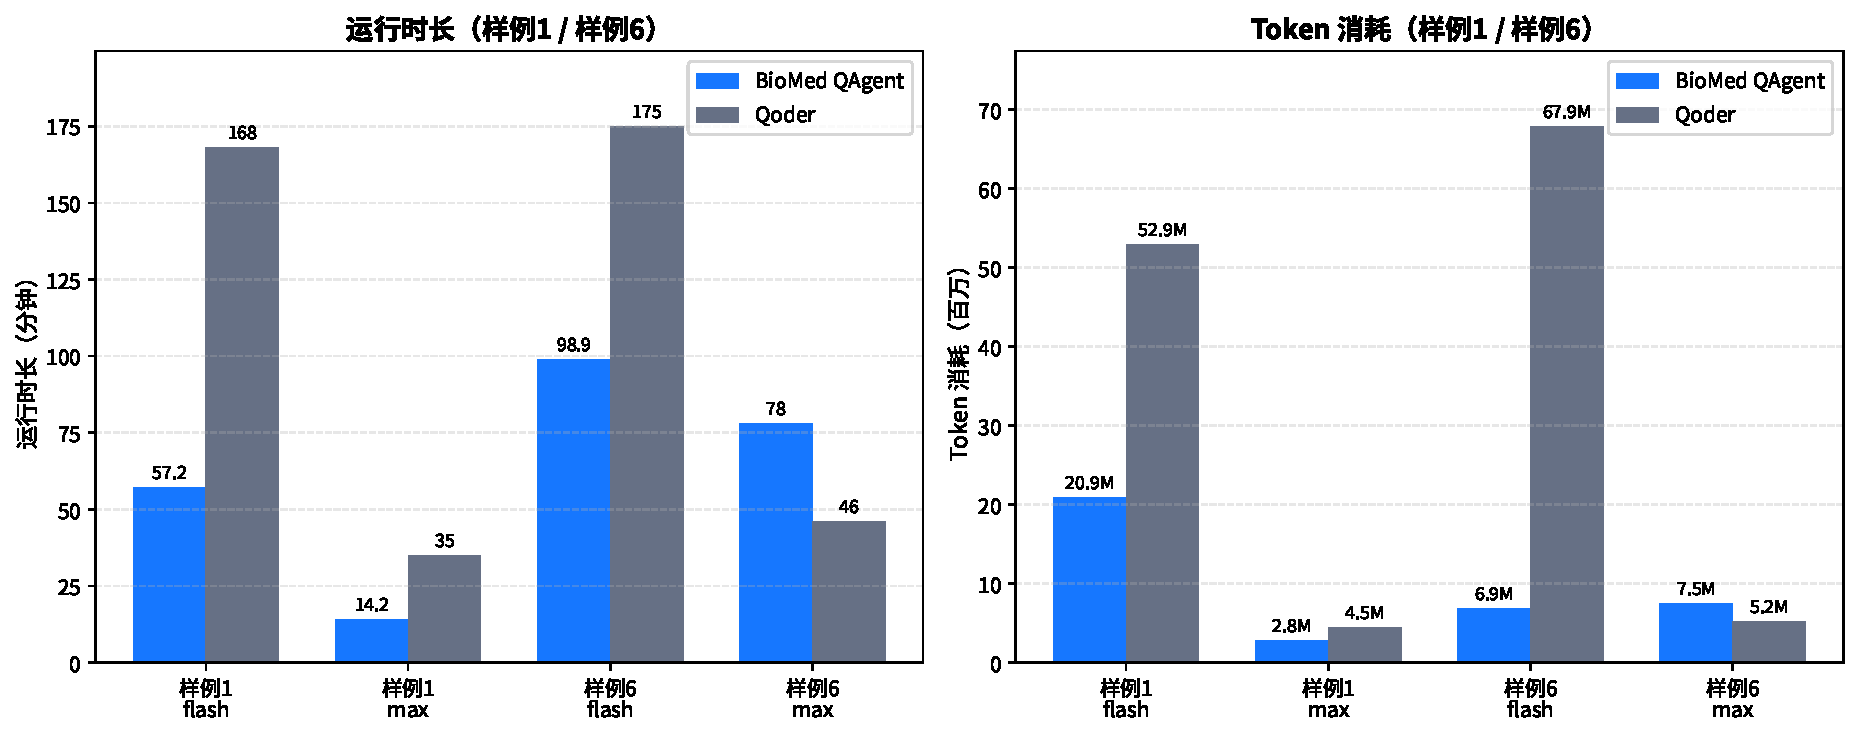
\includegraphics[width=0.97\textwidth]{figures/fig-samples-efficiency-comparison.pdf}
\caption{两案例的运行记录值。来源与计量方式不同，交付内容亦不相同；柱高不能单独用于判断执行效率。}\label{fig:sample-efficiency}
\end{figure}

\subsection{样例1：表达组学数据整合}\label{subsec:gold1-artifact-compare}

需求覆盖按七项任务条目核对：研究纳入、差异表达、样本元数据、平台注释与探针—基因映射、探针水平数据、基因水平数据，以及分析可用性与来源标注。两名评审的记录中，Qoder flash 因探针表仅覆盖16个研究中的5个，该项按部分完成计，总分6.5/7；其余三组为6/7。这个分数不衡量是否查全研究，也不消除纳入研究数的差异。可审计性没有完整四组分项记录，本节仅说明可核对的文件和来源。

\begin{table}[htbp]
\centering
\caption{样例1四组数据产品比较}\label{tab:gold1-artifacts}
\begin{tabularx}{\linewidth}{>{\hsize=0.66000\hsize}L>{\hsize=0.86400\hsize}L>{\hsize=0.90000\hsize}L>{\hsize=1.05600\hsize}L>{\hsize=0.96000\hsize}L>{\hsize=1.56000\hsize}L}
\toprule
\textbf{组} & \textbf{研究数} & \textbf{样本元数据} & \textbf{探针水平} & \textbf{基因水平} & \textbf{证据组织} \\
\midrule
flash · B & 1，GSE86374 & GSM分组支撑表 & 与基因级融合于长表 & 5,294,223行 & 记录级来源定位与发布校验 \\
flash · Q & 16 & 3,226行 & 5个研究宽表 & 13个研究宽表与汇总 & URL、MD5、检索日期、筛选记录 \\
max · B & 2 & GSM分组支撑表 & GSE139038长表 & GSE86374长表 & 记录级来源定位与发布校验 \\
max · Q & 4 & 443行 & 4个研究宽表 & 4个研究宽表 & URL、MD5、质量日志 \\
\bottomrule
\end{tabularx}
\end{table}

交付形态与数据组织。四组产物表现出两种不同的数据组织方式。Qoder 为每个研究输出宽表，每行对应探针或基因、每列对应样本，便于直接进入R 或Python；\mbox{BioMed QAgent} 发布长表，每个样本的每个探针或基因各占一行，并保存记录级来源定位，适合逐行核验和跨来源复用。Qoder flash 纳入16 个研究，\mbox{BioMed QAgent} flash 发布1 个研究，max 发布2 个研究；只有Qoder flash 进一步交付了单研究差异分析和跨研究元分析。

来源定位与质量记录方面，本系统将发布清单与记录定位相连，抽样记录可以定位到原始压缩文件中的具体行；字段类型、单位、映射和溯源检查在发布前执行。样例1 flash 的 GPL6244 探针中，33.3\%没有基因注释，系统保留并标注这些未映射记录。两环境共有记录互查时出现4.1862与4.186等差异，与保留小数位不同相符；由于未核对原始来源，不能据此判定哪一份更准确或证明本系统保留了全部原始精度。

本系统两档均未执行差异表达，纳入研究数也少于 Qoder；记录级溯源还带来存储开销，例如 GSE86374 的规范化日志约0.6 GB。Qoder 以研究宽表及分析结果提供另一种交付形式。本案例呈现了研究范围、表结构、来源粒度和存储成本的取舍，不能仅据总时长认定效率优劣。

运行稳定性。在Qoder flash 运行中，系统发生两次异常中断，由人类手动恢复后继续运行。

\subsection{样例6：文献活性与图表证据}\label{subsec:gold6-artifact-compare}

本案例比较论文与实验记录、补充材料、图表数据，以及来源与置信度说明。由于四组任务条目和证据分项评分尚未全部完成，本节不补填统一覆盖分，而是保留交付结构与离线核对结果。六张表或九件文件只说明发布包的组成，不说明每张表均含有效记录，也不代表已经完成图表曲线数字化。

两份 Qoder 离线包另有结构复用分 X 与证据检查分 Y。X 按模式分解、标识符归一、单位归一、维表、清单和拒绝记录六项取均值；Y 使用来源、定位、清单、方法、检查与原始材料六项。表~\ref{tab:gold6-qoder-2x2}、表~\ref{tab:gold6-qoder-subscores}列出离线评分及其依据。小数分项属于复核者给分，不是数值正确率，也不替代缺少的四组需求评分。

\begin{table}[htbp]
\centering
\caption{样例6两份Qoder离线包的补充评分}\label{tab:gold6-qoder-2x2}
\begin{tabularx}{\linewidth}{>{\hsize=0.55000\hsize}L>{\hsize=0.45000\hsize}L>{\hsize=0.45000\hsize}L>{\hsize=2.55000\hsize}L}
\toprule
\textbf{模型} & \textbf{X} & \textbf{Y} & \textbf{可核对差异} \\
\midrule
flash & 0.950 & 0.808 & 22个CSV；10,682条事实对应10,215个来源位置 \\
max & 0.500 & 0.758 & 结构较紧凑；6,439条事实对应11个来源位置 \\
\bottomrule
\end{tabularx}
\end{table}

\begin{table}[htbp]
\centering
\caption{样例6 Qoder离线包的分项评分}\label{tab:gold6-qoder-subscores}
\begin{tabularx}{\linewidth}{>{\hsize=1.72340\hsize}L>{\hsize=0.63830\hsize}L>{\hsize=0.63830\hsize}L>{\hsize=1.72340\hsize}L>{\hsize=0.63830\hsize}L>{\hsize=0.63830\hsize}L}
\toprule
\textbf{X分项} & \textbf{flash} & \textbf{max} & \textbf{Y分项} & \textbf{flash} & \textbf{max} \\
\midrule
模式分解 & 1.00 & 0.30 & 溯源非空率 & 1.00 & 1.00 \\
标识符归一 & 1.00 & 0.50 & 溯源粒度 & 1.00 & 0.65 \\
单位与剂量归一 & 1.00 & 0.90 & 清单哈希可验证 & 0.60 & 1.00 \\
可复用维表 & 1.00 & 0.10 & 质量检查可复算 & 0.85 & 0.80 \\
清单完整性 & 0.70 & 1.00 & 方法日志深度 & 1.00 & 0.70 \\
拒绝与排除记录 & 1.00 & 0.20 & 原始证据留存 & 0.40 & 0.40 \\
均值 & 0.950 & 0.500 & 均值 & 0.808 & 0.758 \\
\bottomrule
\end{tabularx}
\end{table}

上述分数只描述两份离线包，不能将 X 的0.500视为任务需求覆盖分。表~\ref{tab:gold6-artifacts}进一步列出四组文件结构与可复核内容。

\begin{table}[htbp]
\centering
\caption{样例6四组数据产品的结构与证据}\label{tab:gold6-artifacts}
\begin{tabularx}{\linewidth}{>{\hsize=0.55000\hsize}L>{\hsize=1.15000\hsize}L>{\hsize=1.15000\hsize}L>{\hsize=1.15000\hsize}L}
\toprule
\textbf{组} & \textbf{数据结构} & \textbf{证据与检查} & \textbf{交付内容} \\
\midrule
flash · B & 活性值、实验、论文、补充材料与图表等六个关联表 & 记录级来源与文件摘要 & 当前正式版本共九件文件 \\
flash · Q & 10,682行事实表及筛选、排除、访问记录与维表 & 来源定位较细；清单一处自指摘要不符 & 文件分解较细 \\
max · B & 六个关联表及表结构、溯源和质量评估 & 报告94项检查通过，逐件核验摘要 & 29次模型调用、54次工具调用 \\
max · Q & 6,439行事实表、来源登记与方法日志 & 清单5/5通过；来源定位较粗 & 另含145条GtoPdb策展记录 \\
\bottomrule
\end{tabularx}
\end{table}

交付形态与数据组织。两份Qoder 主表都包含记录编号、突变体、化合物、ChEMBL 标识、活性类型、纳摩尔值、细胞系、来源数据库、检索日期、抽取方法和置信度等核心字段。flash 主表为10,682 $\times$ 109，还提供以摩尔浓度负十进制对数表示的pXC、跨源一致性、化合物身份解析、证据文本以及表格行列坐标；max主表为6,439 $\times$ 35，结构更紧凑，并额外纳入145条GtoPdb（药理学指南数据库）策展记录。flash 还把单剂量筛选、非浓度指标、排除记录、拒绝候选、补充材料访问、未解析附件和参考维表拆为独立文件，这些文件说明它保留了哪些处理结果，不以文件数量代替需求完成程度。

来源定位与质量证据。来源粒度进一步区分了两套产品。flash 的10,682 条事实对应10,215 个不同来源位置，包括ChEMBL 活性标识、表格行列坐标、证据文本和补充材料工作表定位；max 的6,439 条事实只有11 个不同的来源定位值，其中6,285 行共享同一说明。因此，两者来源字段均非空，但flash 更接近记录级定位，max 更接近来源批次级定位。

清单复算方面，Qoder flash 的22个文件在行数、列数和大小上均匹配，21/22个 SHA-1 前缀可验证；清单自指行不匹配，且摘要只保留16位十六进制前缀。其质量检查中，唯一性、正值范围、pXC、一致性分类与来源计数可以复算；部分组合中位数因筛选条件未完整说明，只能复现相对高低。max 的5个清单条目 MD5 全部通过，行列数与来源非空情况也可复算。两份包均缺少方法日志引用的原始响应、附件、图件与提取脚本，无法仅凭离线包重放全过程。

本系统两档将六张关联表及三件说明文件作为当前正式版本交付。flash 先后发布两个版本，第二次明确替代第一次并保留关联；max 记录了94项检查。这样的发布组织便于核对文件、来源和检查结果，但检查数量不代表科学正确率。两环境还存在图表、附件与记录范围差异，本节没有证明同等任务和质量下的效率优势。

\begin{figure}[htbp]
\centering
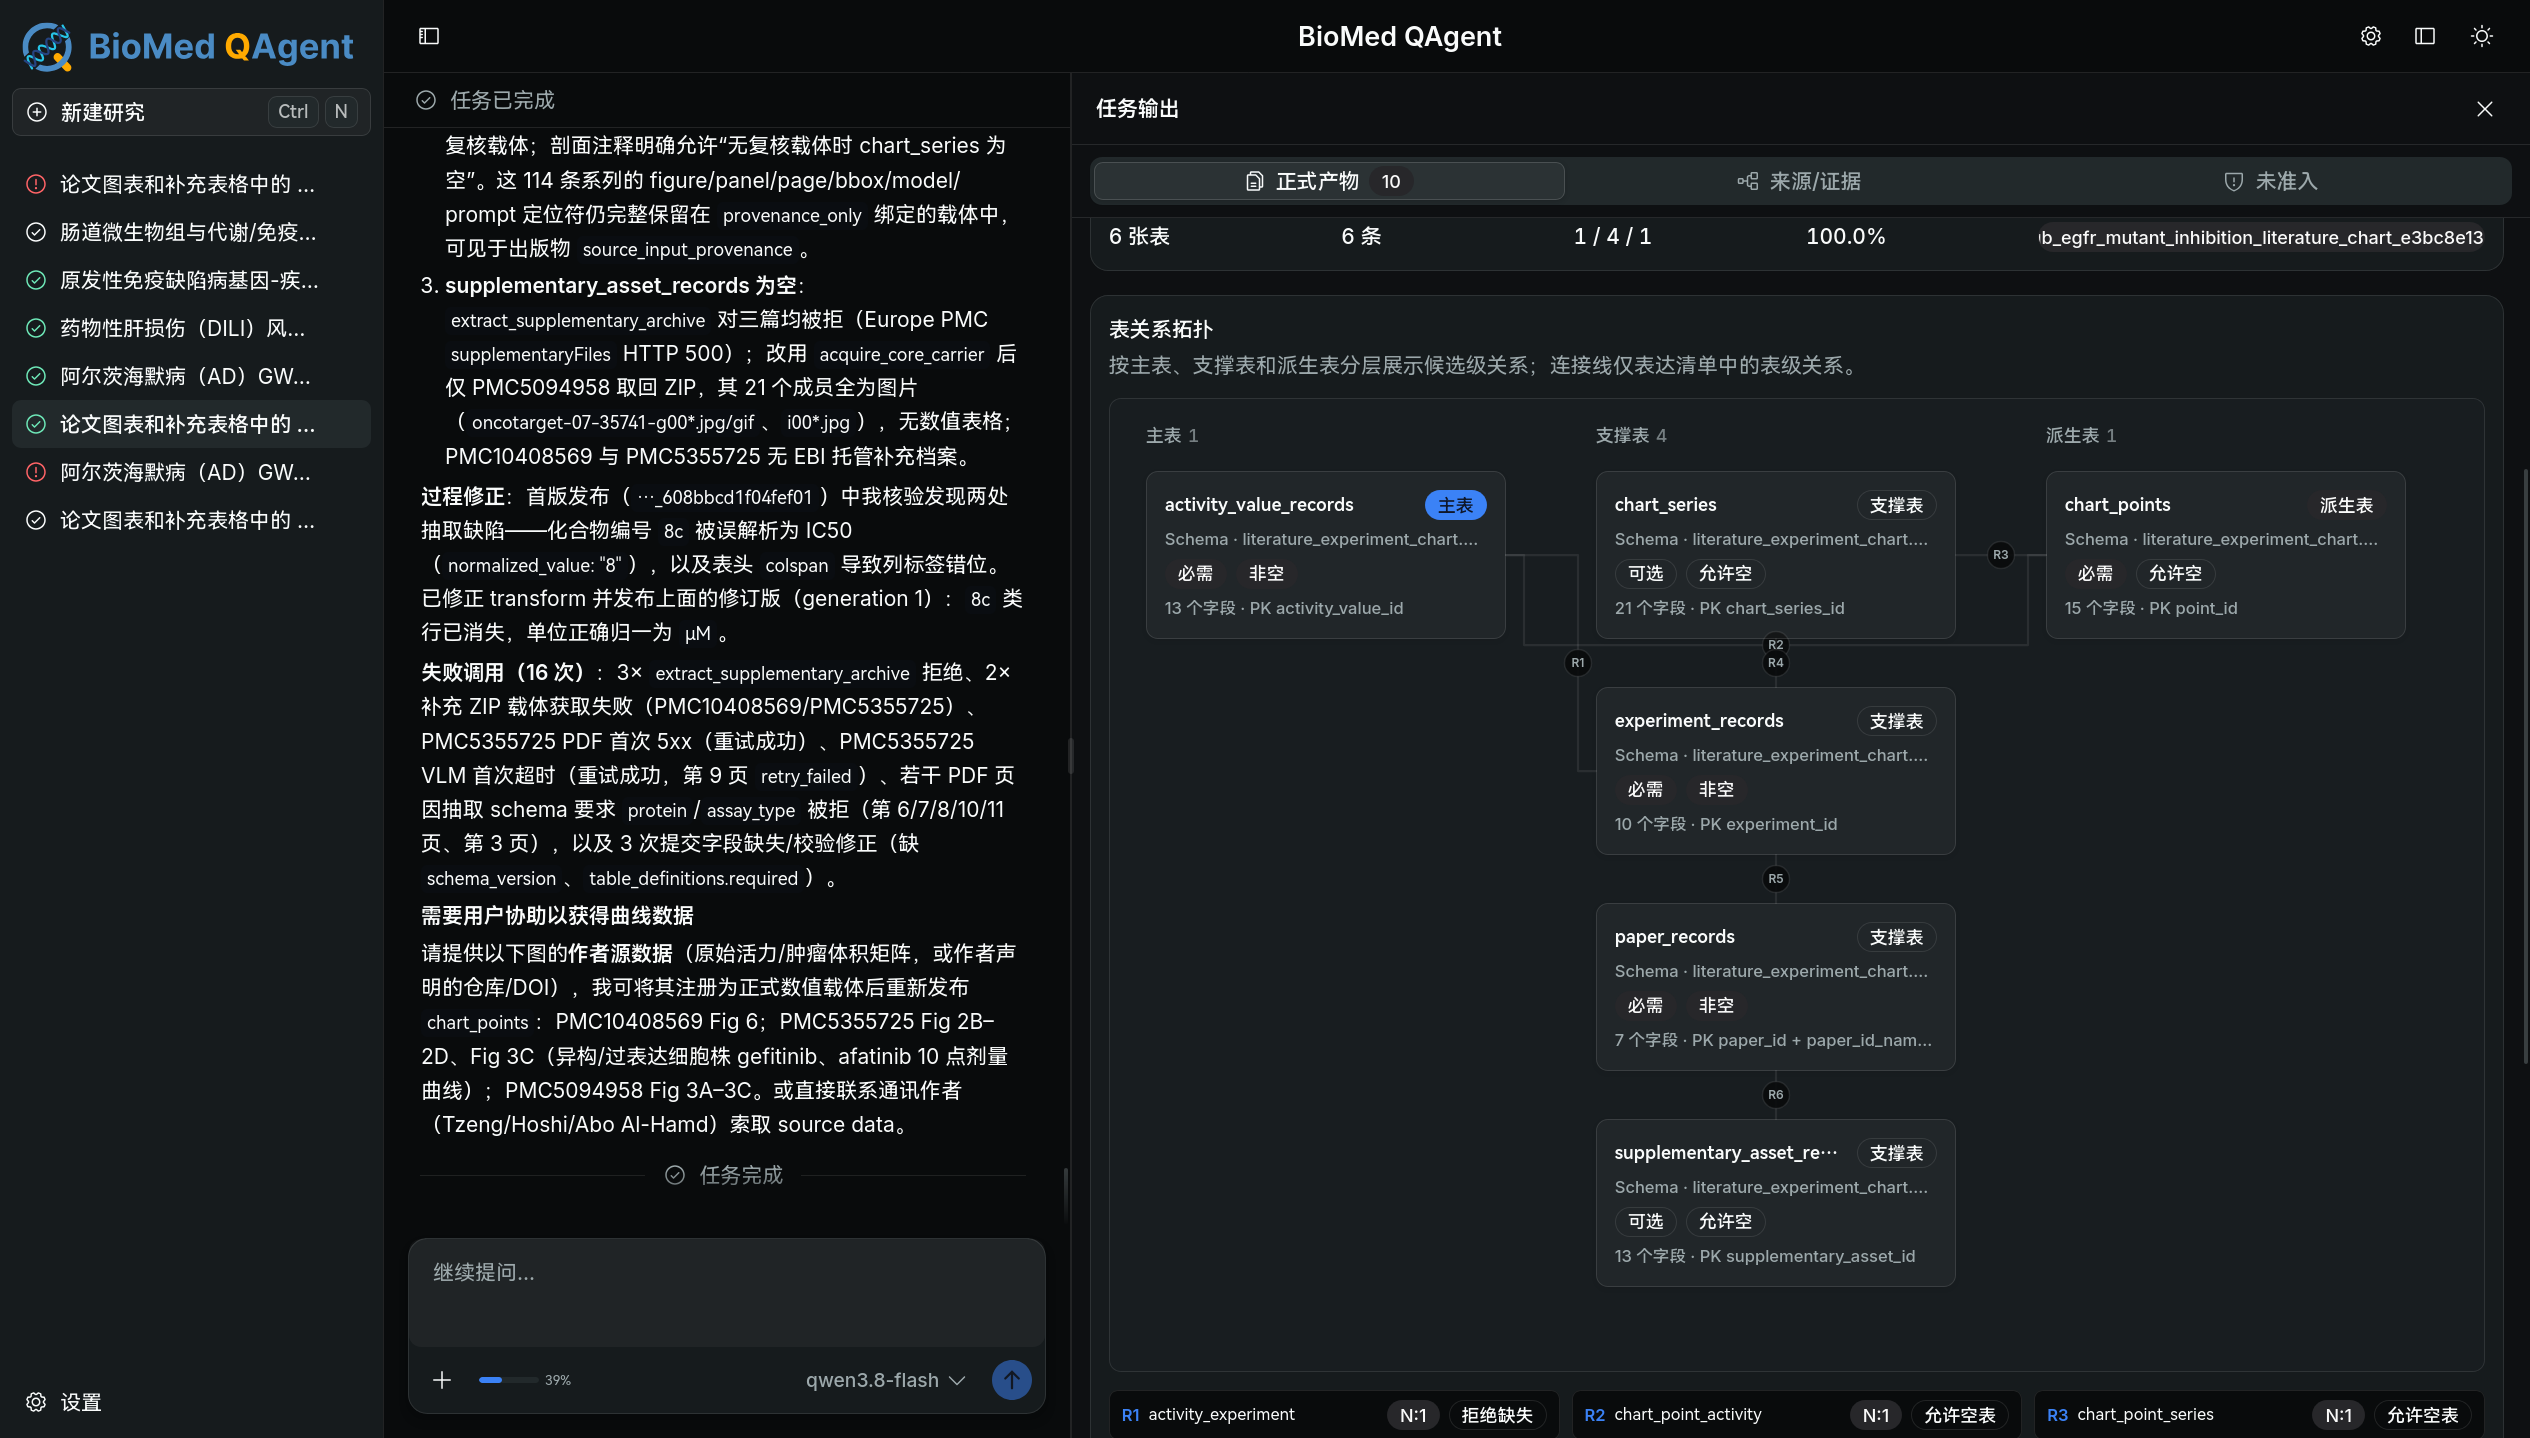
\includegraphics[width=0.93\textwidth]{figures/ui-gold6-table-topology.png}
\caption{样例6正式发布物的表关系与文件组织。}\label{fig:ui-gold6-topology}
\end{figure}

\subsection{主要发现}

首先，本系统将正式发布与可核验文件相连，并在发布前保存字段、关系、来源和质量检查结果。样例1保留未映射探针，样例6组织关联表并保留修改后的发布版本。

其次，文件存在、通过检查和满足原始需求是不同结果。Qoder 的离线包也包含来源与质量记录，不能将它概括为只有聊天回答；本系统的正式发布身份同样不能代替需求覆盖和来源级数值核对。

最后，运行记录显示成本有差异，但交付规模、内容与计量方式尚未统一。较低总量可能同时对应较少交付，不能排除这一解释。本文因此将成本作为观察结果，不据此宣称本系统或某个模型档位更高效。

\section{部署与视频演示}\label{sec:video-demo}

随报告提交的视频演示展示了一次从零开始的独立部署与运行，验证系统不依赖开发环境即可安装和使用：

\begin{enumerate}
  \item 安装与启动：下载正式 release 后运行，无需从源码构建。
  \item 模型配置：在前端设置 qwen3.8-flash 与 API 密钥，界面见图~\ref{fig:ui-settings-models}。
  \item 完全人工审批：演示运行样例7时配置人工审核，流程中出现一次确认，处理后继续并形成正式发布。此演示与表~\ref{tab:gold-overview}的归档运行不是同一次。
  \item 外部来源扩展：配置 ClinicalTrials.gov，查询“2型糖尿病目前有哪些临床试验？给出3个NCT编号、题目和状态”，检查返回字段。该演示只说明这条调用路径，不作为全面检索能力评测。
\end{enumerate}

视频补充了安装、配置、人工处理和继续运行的可见过程。它不补足十二次评测中的全部审批记录，也不证明所有动态发布路径都会自动发起人工验收。

\section{本章小结}

十个案例中，九个至少形成一次正式发布，一个因必需数据缺失而停止；加上两次 max 观察，共十二次运行，十一次正式发布。已交付文件、未完成需求与运行成本分别记录。跨环境比较显示不同系统在研究范围、文件组织和来源定位方面各有差异；当前证据支持描述这些差异，不支持等工作量下的效率排序、科学正确率或查全率结论。

